\documentclass[border=0.2cm]{standalone}
\usepackage{amsmath, amsthm, amssymb, amsfonts}
\usepackage{tikz}
\usepackage{pgfplots}
\usepackage{helvet}
\renewcommand{\familydefault}{\sfdefault}
\usepackage[eulergreek]{sansmath}
\pgfplotsset{
y tick label style = {font=\sansmath\sffamily}}

\begin{document}
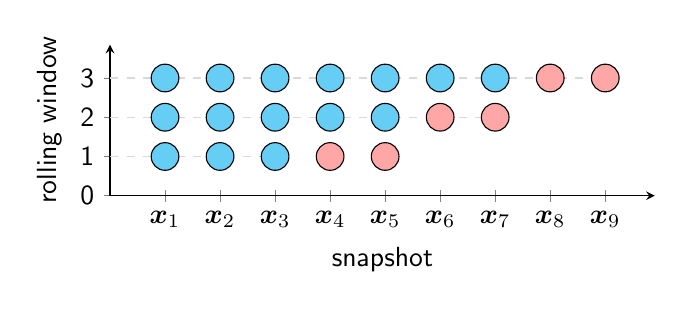
\begin{tikzpicture}
\begin{axis}[axis lines=left, enlargelimits=upper, domain=0:2, xmin=0, ymin=0, ymax=3.5, xtick={1,2,3,4,5,6,7,8,9}, xticklabels={$\boldsymbol{x}_{1}$,$\boldsymbol{x}_{2}$,$\boldsymbol{x}_{3}$,$\boldsymbol{x}_{4}$,$\boldsymbol{x}_{5}$,$\boldsymbol{x}_{6}$,$\boldsymbol{x}_{7}$,$\boldsymbol{x}_{8}$,$\boldsymbol{x}_{9}$}, legend pos=outer north east, width=8.5cm, height=3.5cm, xlabel=snapshot, ylabel=rolling window, xlabel near ticks, ylabel near ticks]
\addplot[only marks, mark size=5, color=cyan!60, draw=black] coordinates{(1,1) (2,1) (3,1)};
\addplot[only marks, mark size=5, color=red!35, draw=black] coordinates{(4,1) (5,1)};
\addplot[only marks, mark size=5, color=cyan!60, draw=black] coordinates{(1,2) (2,2) (3,2) (4,2) (5,2)};
\addplot[only marks, mark size=5, color=red!35, draw=black] coordinates{(6,2) (7,2)};
\addplot[only marks, mark size=5, color=cyan!60, draw=black] coordinates{(1,3) (2,3) (3,3) (4,3) (5,3) (6,3) (7,3)};
\addplot[only marks, mark size=5, color=red!35, draw=black] coordinates{(8,3) (9,3)};
\addplot[dashed, color=gray!30, mark=none] coordinates {(0,1) (3,1)};
\addplot[dashed, color=gray!30, mark=none] coordinates {(0,2) (7,2)};
\addplot[dashed, color=gray!30, mark=none] coordinates {(0,3) (9,3)};
\end{axis}
\end{tikzpicture}
\end{document}
